%!TEX root = ../paper.tex

%%%%%%%%%%%%%%%%%%%%%%
\section{Methodology} \label{sec:methodology}
%%%%%%%%%%%%%%%%%%%%%%


In this section we define the research questions, describe the research
settings, and outline our research method.

\subsection{Research Questions}

Our investigation of code review revolves around the following research
questions, which we iteratively refined during our initial in-field
observations and interviews:

\begin{enumerate}
  \item What are the motivations and expectations for modern code review? Do they change from managers to developers and testers?
  \item What are the actual outcomes of modern code review? Do they match the expectations?
  \item What are the main challenges experienced when performing modern code reviews relative to the expectations and outcomes?
\end{enumerate}

\subsection{Research Setting}

Our study took place with professional developers, testers, and managers.
Microsoft develops software in diverse domains, from high end server enterprise
data management solutions such as SQL Server to mobile phone applications and
smart phone apps to search engines. Each team has its own development culture
and code review policies. Over the past two years, a common tool for code
review at Microsoft has achieved wide-spread adoption. As it represents a
common and growing solution for code review (over 40,000 developers used it so
far), we focused on developers using this tool for code review---\emph{CodeFlow}. 

CodeFlow is a collaborative code review tool that allows users to directly
annotate source code in its viewer and interact with review participants in a
live chat model. The functionality of CodeFlow is similar to other review tools
such Google's Mondrian~\cite{kennedy2006online}, Facebook's Phabricator~\cite{tsotsis2011online} or
open-source Gerrit~\cite{gerrit2012online}. Developers who want their code to
be reviewed create a package with the changed (new, deleted, and modified)
files, select the reviewers, write a message to describe the code review, and
submit everything to the CodeFlow service. CodeFlow then notifies the reviewers
about the incoming task via email.



Once reviewers open a CodeFlow review, they interact with it via a single
desktop window (\figref{fig:codeflow:screenshot}). On the top left (\textbf{1}), they see the list of files
changed in the current submission, plus a ``description.txt'' file, which
contains a textual explanation of the change, written by the author. On bottom
left, CodeFlow shows the list of reviewers and their status (\textbf{2}). We see that
Christian is the review author and Alberto, Tom, and Nachi are the reviewers.
Alberto has reviewed and is waiting for the author to act, as the clock icon
suggests, while Nachi already signed off on the changes. CodeFlow's main view
(\textbf{3}) shows the diff-highlighted content of the file currently under review. Both
the reviewers and the author can highlight portions of the code and add
comments inline (\textbf{4}). These comments can start threads of discussion and are the
interaction points for the people involved in the review. Each user viewing the
same review in CodeFlow sees events as they happen.  Thus, if an author and
reviewer are working on the review at the same time, the communication is
synchronous and comment threads act similar to instant messaging. The comments
are persisted so that if they work at different times, the communication
becomes asynchronous. The bottom right pane (\textbf{5}) shows the summary of all the
comments in the review. 

CodeFlow centralizes and records all the information on code reviews on a
central server. This provides an additional data source that we used to analyze
real code review comments without incurring the Hawthorne effect~\cite{adair1984hawthorne}.



\begin{figure}[t] %  figure placement: here, top, bottom, or page
   \centering
   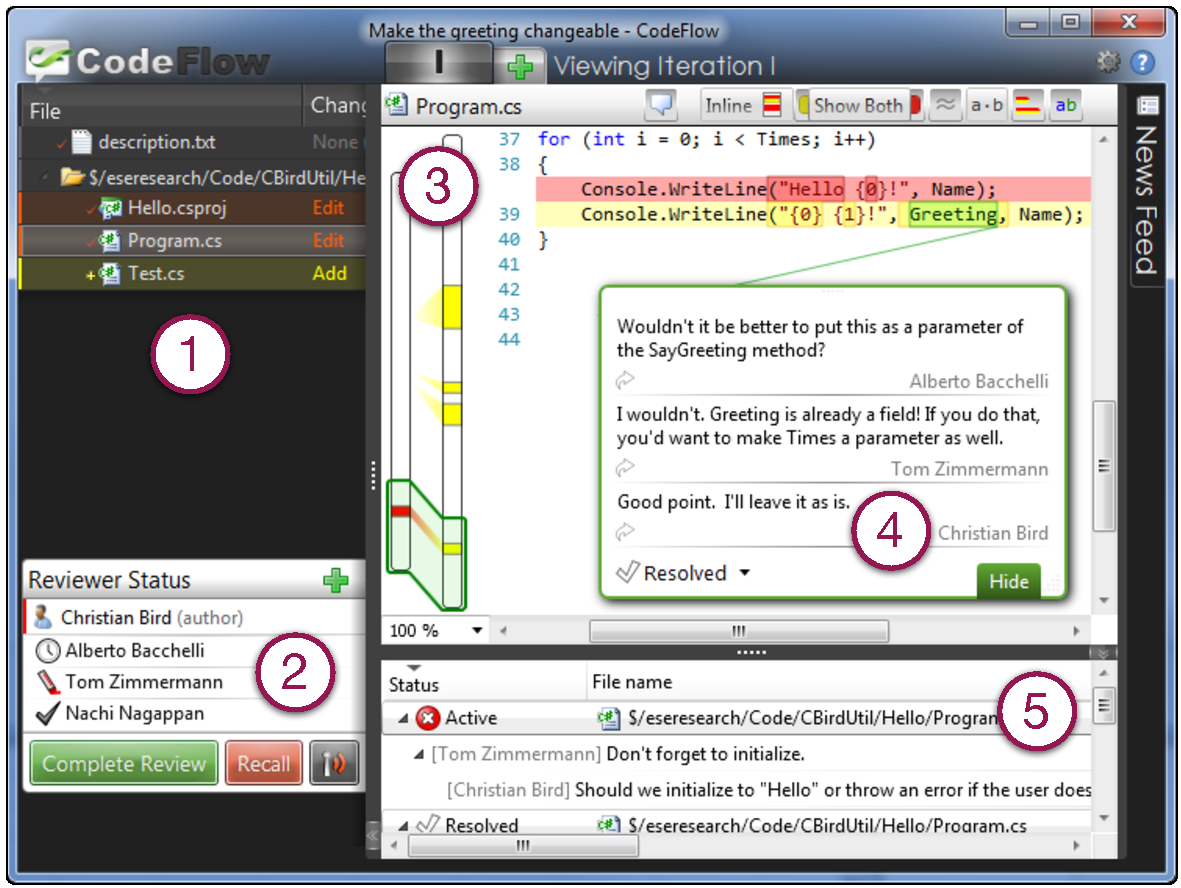
\includegraphics[width=0.98\columnwidth]{codeflow.pdf}
   \caption{CodeFlow, the main code review tool used by developers at Microsoft.}
   \label{fig:codeflow:screenshot}
      \vspace{-1.5em}
\end{figure}



\subsection{Research Method}

\begin{figure*}[t] %  figure placement: here, top, bottom, or page
   \centering
   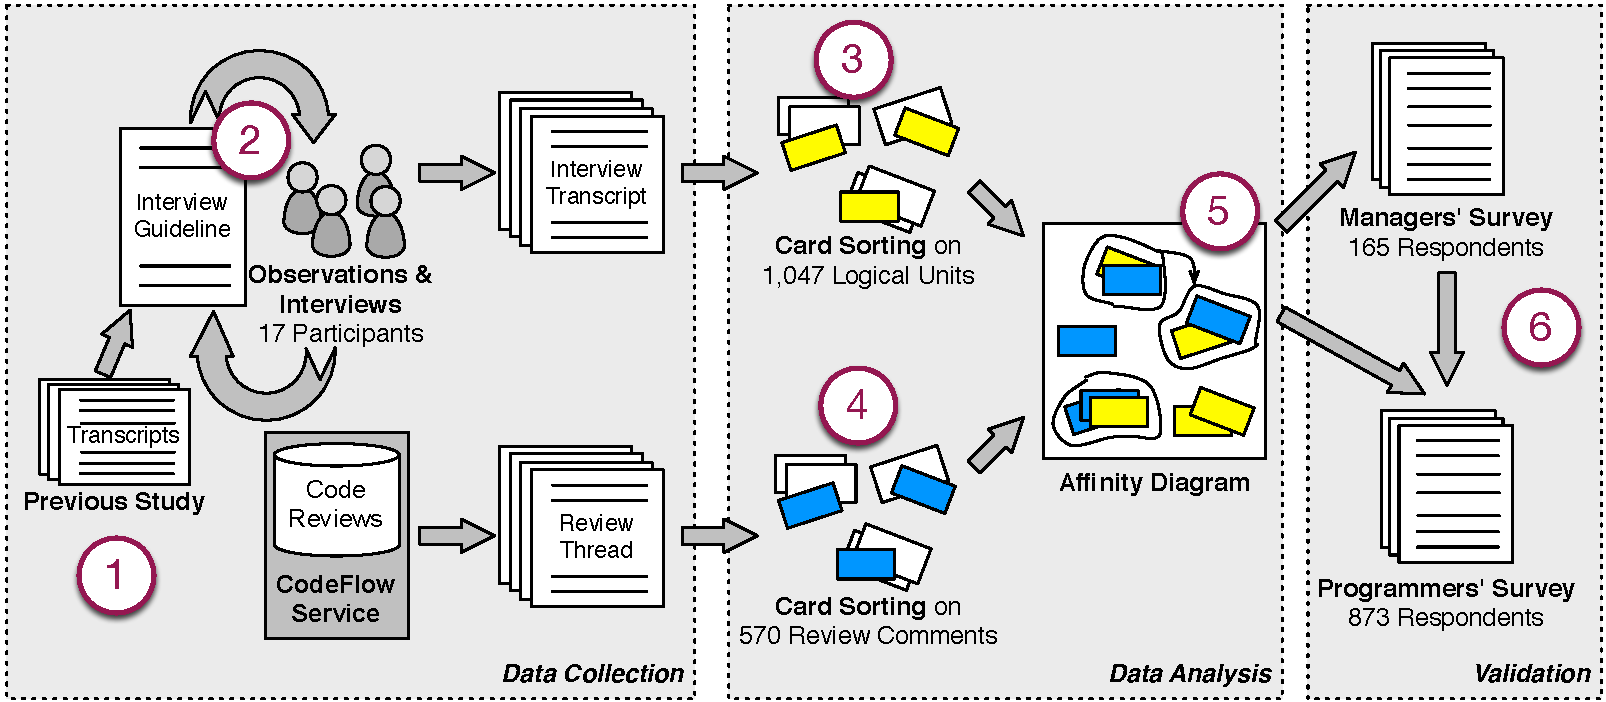
\includegraphics[width=1.4\columnwidth]{methodology.pdf}
   \caption{The mixed approach research method applied.}
   \label{fig:research-method}
   \vspace{-1.5em}
\end{figure*}

Our research method followed a mixed approach~\cite{creswell2009research}, depicted in
\figref{fig:research-method}, collecting data from different sources for triangulation: (\textbf{1})
analysis of previous study, (\textbf{2}) observations and interviews with developers,
(\textbf{3}) card sort on interview data,  (\textbf{4}) card sort on code review comments, (\textbf{5})
the creation of an affinity diagram, and (\textbf{6}) survey to managers and
programmers.

\textbf{1. Analysis of previous study:} Our research started with the analysis of a
study commissioned by Microsoft, between April and May 2012 carried out by an
external vendor. The study investigated how different product teams were using
CodeFlow. It consisted of structured interviews (lasting 30-50 minutes) to 23
people with different roles.

Most of the interview questions revolved around topics that are very specific
to tool usage, and were only tangentially related to this work. We found one
relevant as a starting point for our study: ``\emph{What do you hope to accomplish
when you submit a code review?}'' We analyzed the transcript of this answer, for
each interview, through the process of \emph{coding}~\cite{berg2004qualitative} (also used in
\emph{grounded theory}~\cite{adolph2011using}): breaking up the answers into smaller coherent
units (sentences or paragraphs) and adding \emph{codes} to them. We organized codes
into \emph{concepts}, which in turn were grouped into more abstract \emph{categories}.

From this analysis, four motivations emerged for code review: finding defects,
maintaining team awareness, improving code quality, and assessing the
high-level design. We used them to draw an initial guideline for our
interviews.

\textbf{2. Observations and interviews with developers:} Next, we conducted a series of
one-to-one meetings with developers who use CodeFlow, each taking 40-60
minutes. 

We contacted 100 randomly selected candidates who signed-off between 50 and 250 code
reviews since the CodeFlow release and sampled across different product teams
to address our research questions from a \emph{multi-point} perspective. We wrote
developers who used CodeFlow in the past and asked them to contact us, giving
us 30 minute notice when they received their next review task so that we could
observe.  The respondents that we interviewed comprised five developers, four
senior developers, six testers, one senior tester, and one software architect.
Their time in the company ranged from 18 months to almost 10 years, with a
median of five years. 

Each meeting was comprised of two parts: In the first part, we observed them
performing the code review that they had been assigned. To minimize
invasiveness and the Hawthorne effect, we used only one observer, and to encourage the participant to
narrate their work, we asked the participants to consider him as a newcomer to
the team. In this way, most developers thought aloud without need of prompting.
With consent, we recorded the audio, assuring the participants of anonymity.
Since we, as observers, have backgrounds in software development and practices
at Microsoft, we could understand most of the work and where and how
information was obtained without inquiry. 

The second part of the meeting was a \emph{semi-structured} interview~\cite{taylor2010qualitative}. Semi-structured interviews make use of an \emph{interview guide} that
contains general groupings of topics and questions rather than a pre-determined
exact set and order of questions.  They are often used in an exploratory
context to ``find out what is happening [and] to seek new insights''~\cite{weiss1995learning}. 
The guideline was iteratively refined after each interview, in
particular when developers started providing answers very similar to the
earlier ones, thus reaching a saturation effect.

After the first 5-6 meetings, the observations reached a \emph{saturation} point~\cite{Glas1998a}: They were providing insights very similar to the earlier ones. For this, we adjusted the meetings to have shorter observations, which we used as a starting point for our meetings and as a ``hook'' to talk about topics in our guideline.

The audio of each interview was then transcribed and broken up into smaller
coherent units for subsequent analysis.

\textbf{3. Card sort (meetings):} To group codes that emerged from interviews and
observations into categories, we conducted a \emph{card sort}. Card sorting is a
sorting technique that is widely used in information architecture to create
mental models and derive taxonomies from input data~\cite{barker2005online}. In our case
it helped to organize the codes into hierarchies to deduce a higher level of
abstraction and identify common themes. A card sort involves three phases: In
the \begin{inparaenum}[(1)]
\item \emph{preparation phase}, participants of the card sort are selected and the
cards are created; in the 
\item \emph{execution phase}, cards are sorted into meaningful
groups with a descriptive title; and in the 
\item \emph{analysis phase}, abstract hierarchies are formed to deduce general categories.
\end{inparaenum}

We applied an \emph{open card sort}: There were no predefined groups. Instead, the
groups emerged and evolved during the sorting process. In contrast, a closed
card sort has predefined groups and is typically applied when themes are known
in advance, which was not the case for our study.

The first author of this paper created all of the cards, from the 1,047
coherent units in the interviews. Throughout our further analysis other
researchers (the second author and external people) were involved in developing
categories and assigning cards to categories, so as to strengthen the validity
of the result. The first author played a special role of ensuring that the
context of each question was appropriately considered in the categorization,
and creating the initial categories. To ensure the integrity of our categories,
the cards were sorted by the first author several times to identify initial
themes. To reduce bias from the first author sorting the cards to form initial themes, all researchers reviewed and agreed on the final set of
categories.

\textbf{4. Card sort (code review comments):} The same method was applied to group code
review comments into categories: We randomly sampled 200 threads with at least
two comments (e.g., Point 4 of \figref{fig:research-method}), from the entire dataset of CodeFlow
reviews, which embeds data from dozens of independent software products at
Microsoft. We printed one card for each comment (along with the entire
discussion thread to give the context), totaling 570 cards, and conducted a
card sort, as performed for the interviews, to identify common themes.

\textbf{5. Affinity Diagram:} We used an \emph{affinity diagram} to organize the categories
that emerged from the card sort. This tool allows large numbers of ideas to be
sorted into groups for review and analysis~\cite{shade2000improving}. We used it
to generate an overview of the topics that emerged from the card sort, in order
to connect the related concepts and derive the main themes. For generating the
affinity diagram, we followed the five canonical steps: we \begin{inparaenum}[(1)] 
\item recorded the categories on post-it-notes, 
\item spread them onto a wall, 
\item sorted the categories based on discussions, until all are sorted and all participants agreed, 
\item named each group, and 
\item captured and discussed the themes.
\end{inparaenum}


\textbf{6. Surveys:} The final step of our study was aimed at validating the
concepts that emerged from the previous phases. Towards this goal, we created
two surveys to reach a significant number of participants and to challenge our
conclusions (The full surveys are available as a technical report~\cite{bacchelli2012appendix}). 
For the design of the surveys, we followed Kitchenham and
Pfleeger's guidelines for personal opinion surveys~\cite{kitchenham2008personal}. 
Both surveys were anonymous to increase response rates~\cite{tyagi1989effects}.

We sent the first survey to a cross section of managers.  We considered
managers for which at least half of their team performed code reviews regularly
(on average, one per week or more) and sampled along two dimensions.  The first
dimension was whether or not the manager had participated in a code review
himself since the beginning of the year and the second dimension was whether
the manager managed a single team or multiple teams (a manager of managers).
Thus, we had one sample of first level managers who participated in review,
another sample of second level managers who participated in reviews, \etc  The
first survey was a short survey comprising 6 questions (all optional), which we
sent to 600 managers that had at least 10 direct or indirect reporting
developers who used CodeFlow. The central focus was the open
question asking to enumerate the main motivations for doing code reviews in
their team. We received 165 answers (28\% response rate), which we analyzed
before devising the second survey.

The second survey comprised 18 questions, mostly closed with multiple choice
answers, and was sent to 2,000 randomly chosen developers who signed off on
average at least one code review per week since the beginning of the year. We
used the time frame of January to June of 2012 to minimize the amount of
organizational churn during the time period and identify employees' activity in
their current role and team.  We received 873 answers (44\% response rate). Both
response rates were  high, as other online surveys in software engineering have
reported response rates ranging from 14\% to 20\%~\cite{punter2003conducting}.




